\documentclass{beamer}
\usetheme{Madrid}
\usecolortheme{default}
\graphicspath{{figures/}{../outputs/figures/}{paper/figures/}{outputs/figures/}}

\title[Fairness Metrics Under Shift]
{When Fairness Metrics Disagree Under Shift: A Stylized Case Study of a Medical Follow-up Risk Score under Hospital Deployment Shift}

\subtitle{When a ``fair'' hospital model travels and quietly becomes unfair.}

\author[Group 0]{Meixuan Chen}

\institute[ ]{Department of Electrical and Computer Engineering}

\date[Algorithmic Fairness] 
{Algorithmic Fairness Seminar -- Summer 2026}

%\logo{\includegraphics[height=0.8cm]{logo_uoft}}

\definecolor{uoftblue}{RGB}{6,41,88}
\setbeamercolor{titlelike}{bg=uoftblue}
\setbeamerfont{title}{series=\bfseries}

\begin{document}

\frame{\titlepage}


\begin{frame}
\frametitle{Motivation: Fairness Metrics in Practice}

\begin{itemize}
    \item Group fairness metrics (e.g., demographic parity, equalized odds) are \alert{defined under a fixed data-generating process}.
    \item Real-world deployments are rarely stable---especially when risk scores are moved across hospitals or regions.
    \item A hospital may monitor \alert{one} fairness metric (e.g., demographic parity) and implicitly assume other notions of equity move in the same direction.
\end{itemize}

\vspace{0.15cm}

\small
\textbf{This project asks (RQ1--RQ3):}
\begin{enumerate}
    \item How do standard group fairness metrics behave under controlled shifts, even when the underlying classifier remains fixed?
    \item When demographic parity and error-based metrics disagree, does the discrepancy reflect degradation in clean outcomes or measurement distortion induced by recorded-label noise?
    \item How do the three mitigation strategies change fairness metrics and utility?
\end{enumerate}

\end{frame}


\begin{frame}
\frametitle{Method: Distribution Shift Mechanisms}

\begin{enumerate}
    \item \textbf{Group-conditioned base-rate shift:} Varies group-specific prevalence.
    \small
    \begin{itemize}
        \item $\Pr(Y=1 \mid S=0) = 0.3 + 0.2\alpha$, $\Pr(Y=1 \mid S=1) = 0.3 - 0.2\alpha$, $\alpha \in [0,1]$.
        \item Mimics different disease prevalence across groups in the target hospital.
    \end{itemize}
    
    \item \textbf{Group-specific covariate shift:} Changes feature scale for one group.
    \begin{itemize}
        \item Multiplicative factor $\gamma \in [1,4]$ on informative feature $X_1$.
        \item Preserves $P(Y \mid X,S)$; mimics case-mix or feature-distribution differences.
    \end{itemize}
    
    \item \textbf{Group-specific label noise shift:} Flips labels asymmetrically.
    \begin{itemize}
        \item Positive labels in group A flipped with prob. $\beta \in [0,0.3]$.
        \item Negative labels in group B flipped with prob. $\beta/2$.
        \item Mimics asymmetric diagnostic coding errors.
    \end{itemize}
\end{enumerate}

\textit{Full constructions in Appendix.}

\end{frame}


\begin{frame}
\frametitle{Method: Fairness and Calibration Metrics}
\begin{block}{Demographic Parity Difference (DP diff)}
\[
|\Pr(\hat{Y}=1 \mid S=0) - \Pr(\hat{Y}=1 \mid S=1)|
\]
\small Measures balance in positive prediction rates across groups.
\end{block}

\begin{block}{Equalized Odds Difference (EO diff)}
\[
\max\big(|\text{TPR}_0 - \text{TPR}_1|, |\text{FPR}_0 - \text{FPR}_1|\big)
\]
\small Worst-case discrepancy in both true and false positive rates.
\end{block}

\begin{block}{True-Positive-Rate Gap (TPR gap)}
\[
|\text{TPR}_0 - \text{TPR}_1|
\]
\small Equal-opportunity violation relative to the chosen outcome definition.
\end{block}

\tiny
Also track Expected Calibration Error (ECE) globally and per-group; report ECE gap.

\end{frame}


\begin{frame}
\frametitle{Method: Mitigation Strategies}

Three interventions, each representing a distinct target-data access regime:

\vspace{0.3cm}

\begin{enumerate}
    \item \textbf{KDE Importance Reweighting:}
    \begin{itemize}
        \item Estimates density ratio $w(x)=\hat{p}_{\text{target}}(x)/\hat{p}_{\text{train}}(x)$.
        \item Reweights logistic loss; justified under pure covariate shift.
    \end{itemize}
    
    \item \textbf{Post-hoc Threshold Adjustment (Equal Opportunity):}
    \begin{itemize}
        \item Uses labeled target calibration set $(X,\tilde{Y},S)$.
        \item Matches the larger group TPR observed at threshold 0.5.
    \end{itemize}
    
    \item \textbf{Target-Distribution Retraining:}
    \begin{itemize}
        \item Retrains same model on labeled target sample $(X,\tilde{Y})$.
        \item Supervised reference, not a fairness-specific fix.
    \end{itemize}
\end{enumerate}

\end{frame}


\begin{frame}
\frametitle{Experimental Setup}

\textbf{Data and Models:}
\begin{itemize}
    \item Source training, shifted evaluation, target retraining: $N=5000$ each.
    \item KDE adaptation and threshold calibration: $N=1000$ each.
    \item Classifier: correctly specified logistic regression on $X=(X_1,X_2)$ without $S$ ($\text{max\_iter}=1000$, default L2, $C=1.0$).
    \item Fairness metrics via \texttt{fairlearn.metrics}; ECE with 10 bins.
    \item \alert{Results averaged over 3 seeds for one-dimensional sweeps, 5 seeds for the danger-zone grid; bands show $\pm 1$ standard deviation.}
\end{itemize}

\vspace{0.3cm}

\textbf{Shift Parameter Grids:}
\begin{itemize}
    \item Base-rate shift: $\alpha \in [0, 1]$, 11 steps.
    \item Covariate shift: $\gamma \in [1, 4]$, 10 steps.
    \item Label noise: $\beta \in [0, 0.3]$, 10 steps.
    \item Joint $(\alpha,\beta)$ grid: $11 \times 10 = 110$ cells.
\end{itemize}

\end{frame}

\begin{frame}
\frametitle{Results: One-Dimensional Metric Behaviour}
\centering
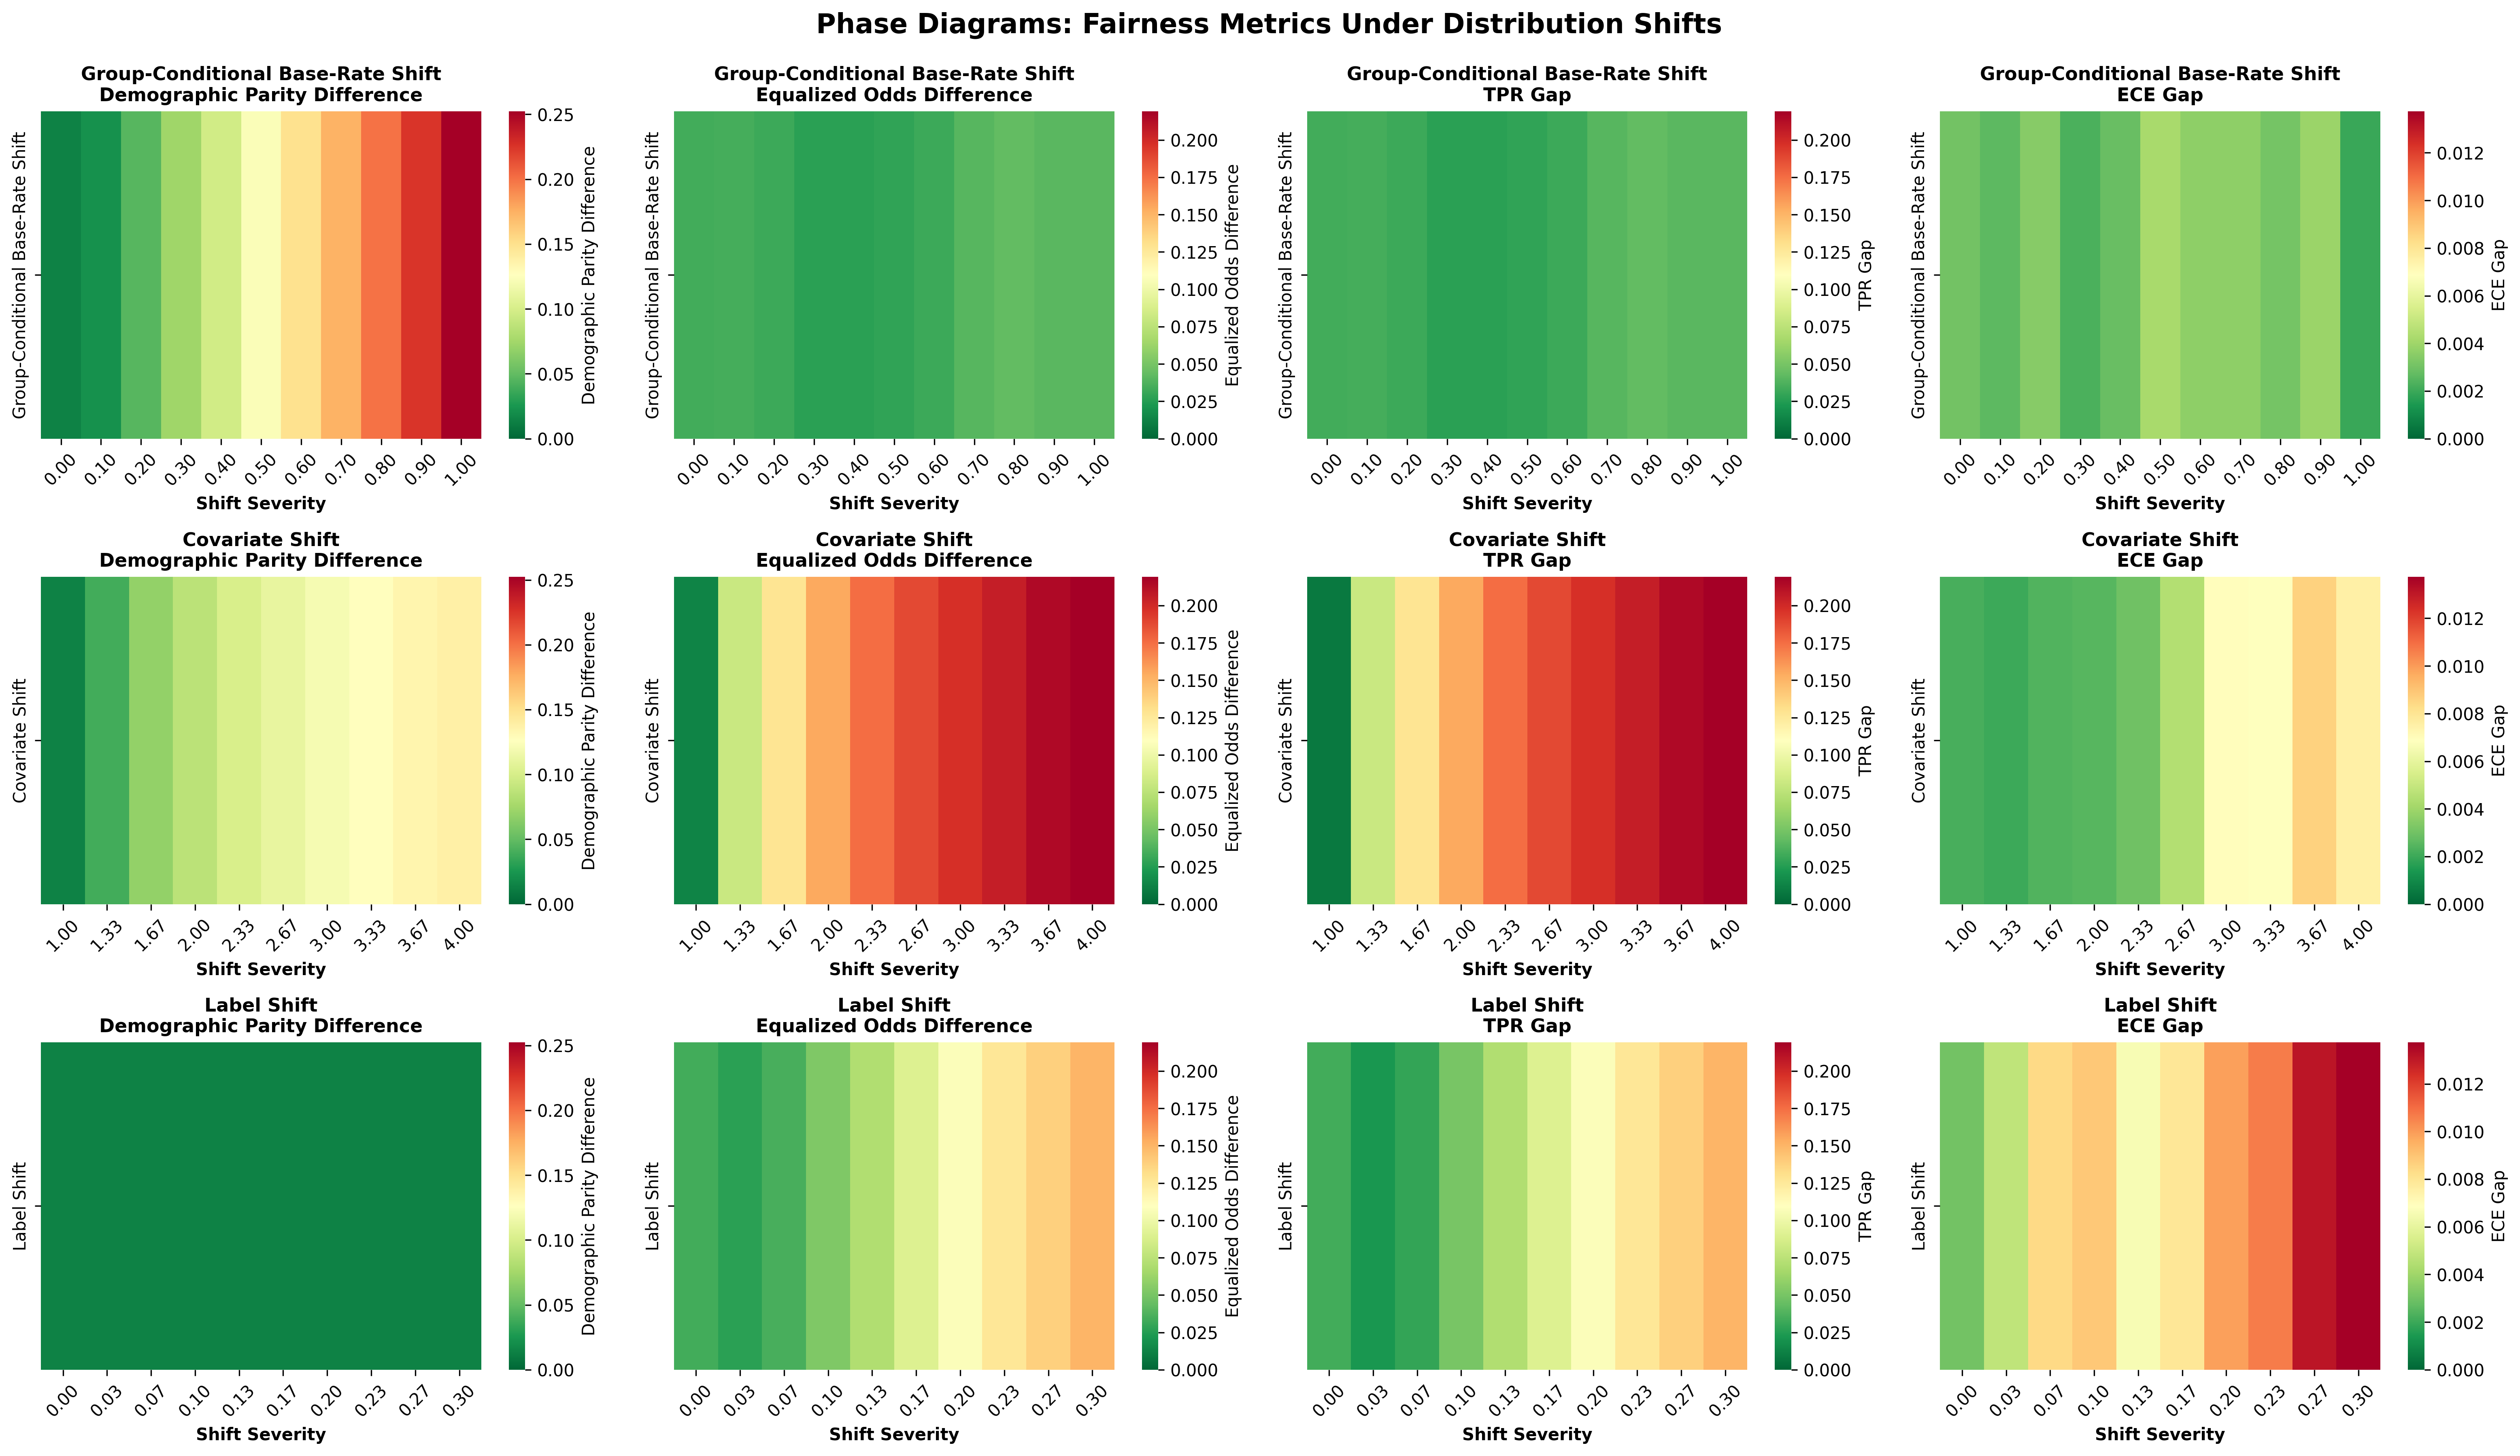
\includegraphics[width=0.88\textwidth]{phase_diagrams.png}
\par\smallskip
{\scriptsize\itshape Figure S2: Three-seed mean metrics versus shift severity.}
\end{frame}


\begin{frame}
\frametitle{Results: Key Empirical Findings (Part 1)}
\small

\textbf{Group-conditioned base-rate shift:}
\begin{itemize}
    \item DP increases from $0.014$ to $0.252$ as $\alpha$ goes from 0 to 1.
    \item TPR gap remains between $0.027$ and $0.043$.
    \item \alert{Metrics react very differently to the same prevalence change.}
\end{itemize}

\vspace{0.1cm}

\textbf{Pure covariate shift:}
\begin{itemize}
    \item DP reaches $0.139$, EO reaches $0.219$, TPR gap reaches $0.219$ at $\gamma=4$.
    \item ECE gap remains below $0.009$---\alert{little between-group calibration disparity}.
    \item Metrics worsen but at different rates; they do not signal identical concern.
\end{itemize}

\vspace{0.1cm}

\textbf{Asymmetric label noise:}
\begin{itemize}
    \item DP stays flat at $0.014$.
    \item Recorded-label TPR gap worsens from $0.034$ to $0.150$.
    \item Clean-outcome TPR gap remains $0.034$---\alert{the apparent degradation is measurement distortion}.
\end{itemize}

\end{frame}


\begin{frame}
\frametitle{Results: The Danger Zone (Joint Prior + Label Noise)}
\small
Define relative to the no-shift cell:
\[
\Delta_D = \text{DP}(\alpha,\beta)-\text{DP}(0,0),\quad
\Delta_T = \text{TPRGap}_{\tilde{Y}}(\alpha,\beta)-\text{TPRGap}_{\tilde{Y}}(0,0).
\]
The \emph{metric-monitoring danger zone} rule is
\[
\Delta_T \ge 0.05 \;\land\; \big[\,\Delta_D \le 0.02 \;\lor\; \Delta_T \ge 2\max(\Delta_D,0)\,\big].
\]
\begin{columns}[T,onlytextwidth]
    \begin{column}{0.66\textwidth}
        \centering
        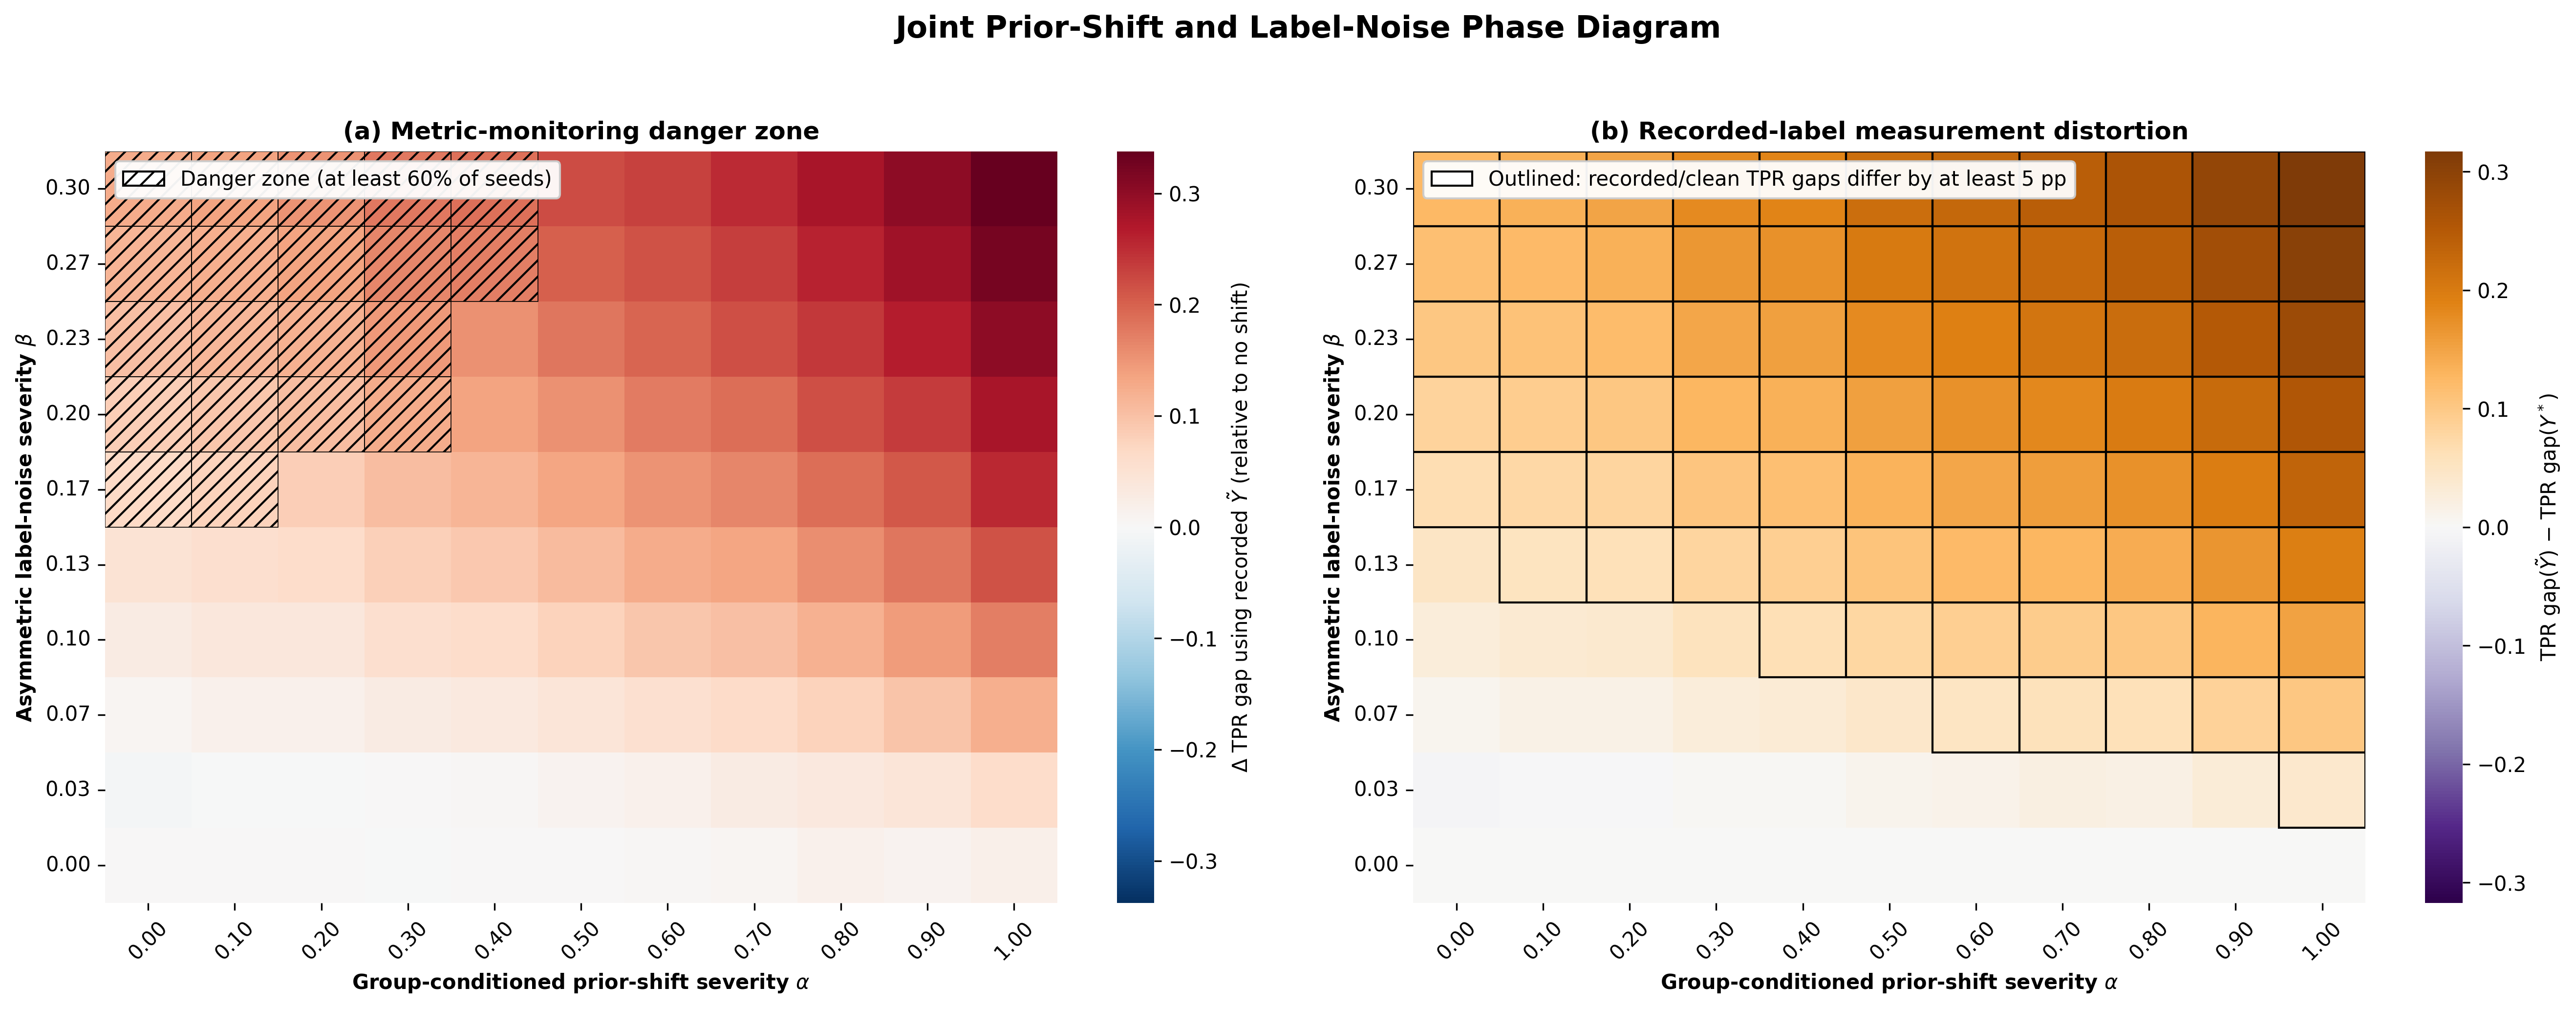
\includegraphics[width=\linewidth]{danger_zone_phase_diagram.png}
        \par\smallskip
        {\scriptsize\itshape Figure 1: Hatched cells satisfy the rule in at least 3 of 5 seeds; panel (b) compares recorded and clean TPR gaps.}
    \end{column}
    \begin{column}{0.31\textwidth}
        \scriptsize
        \begin{itemize}
            \item 20 of 110 cells are dangerous, beginning near $\beta=0.17$ at low $\alpha$.
            \item 78 cells differ by at least five points between clean and recorded TPR gaps.
            \item Sensitivity variants retain 12--31 danger cells.
        \end{itemize}
    \end{column}
\end{columns}

\end{frame}


\begin{frame}
\frametitle{Results: Mitigation Comparison}
\centering
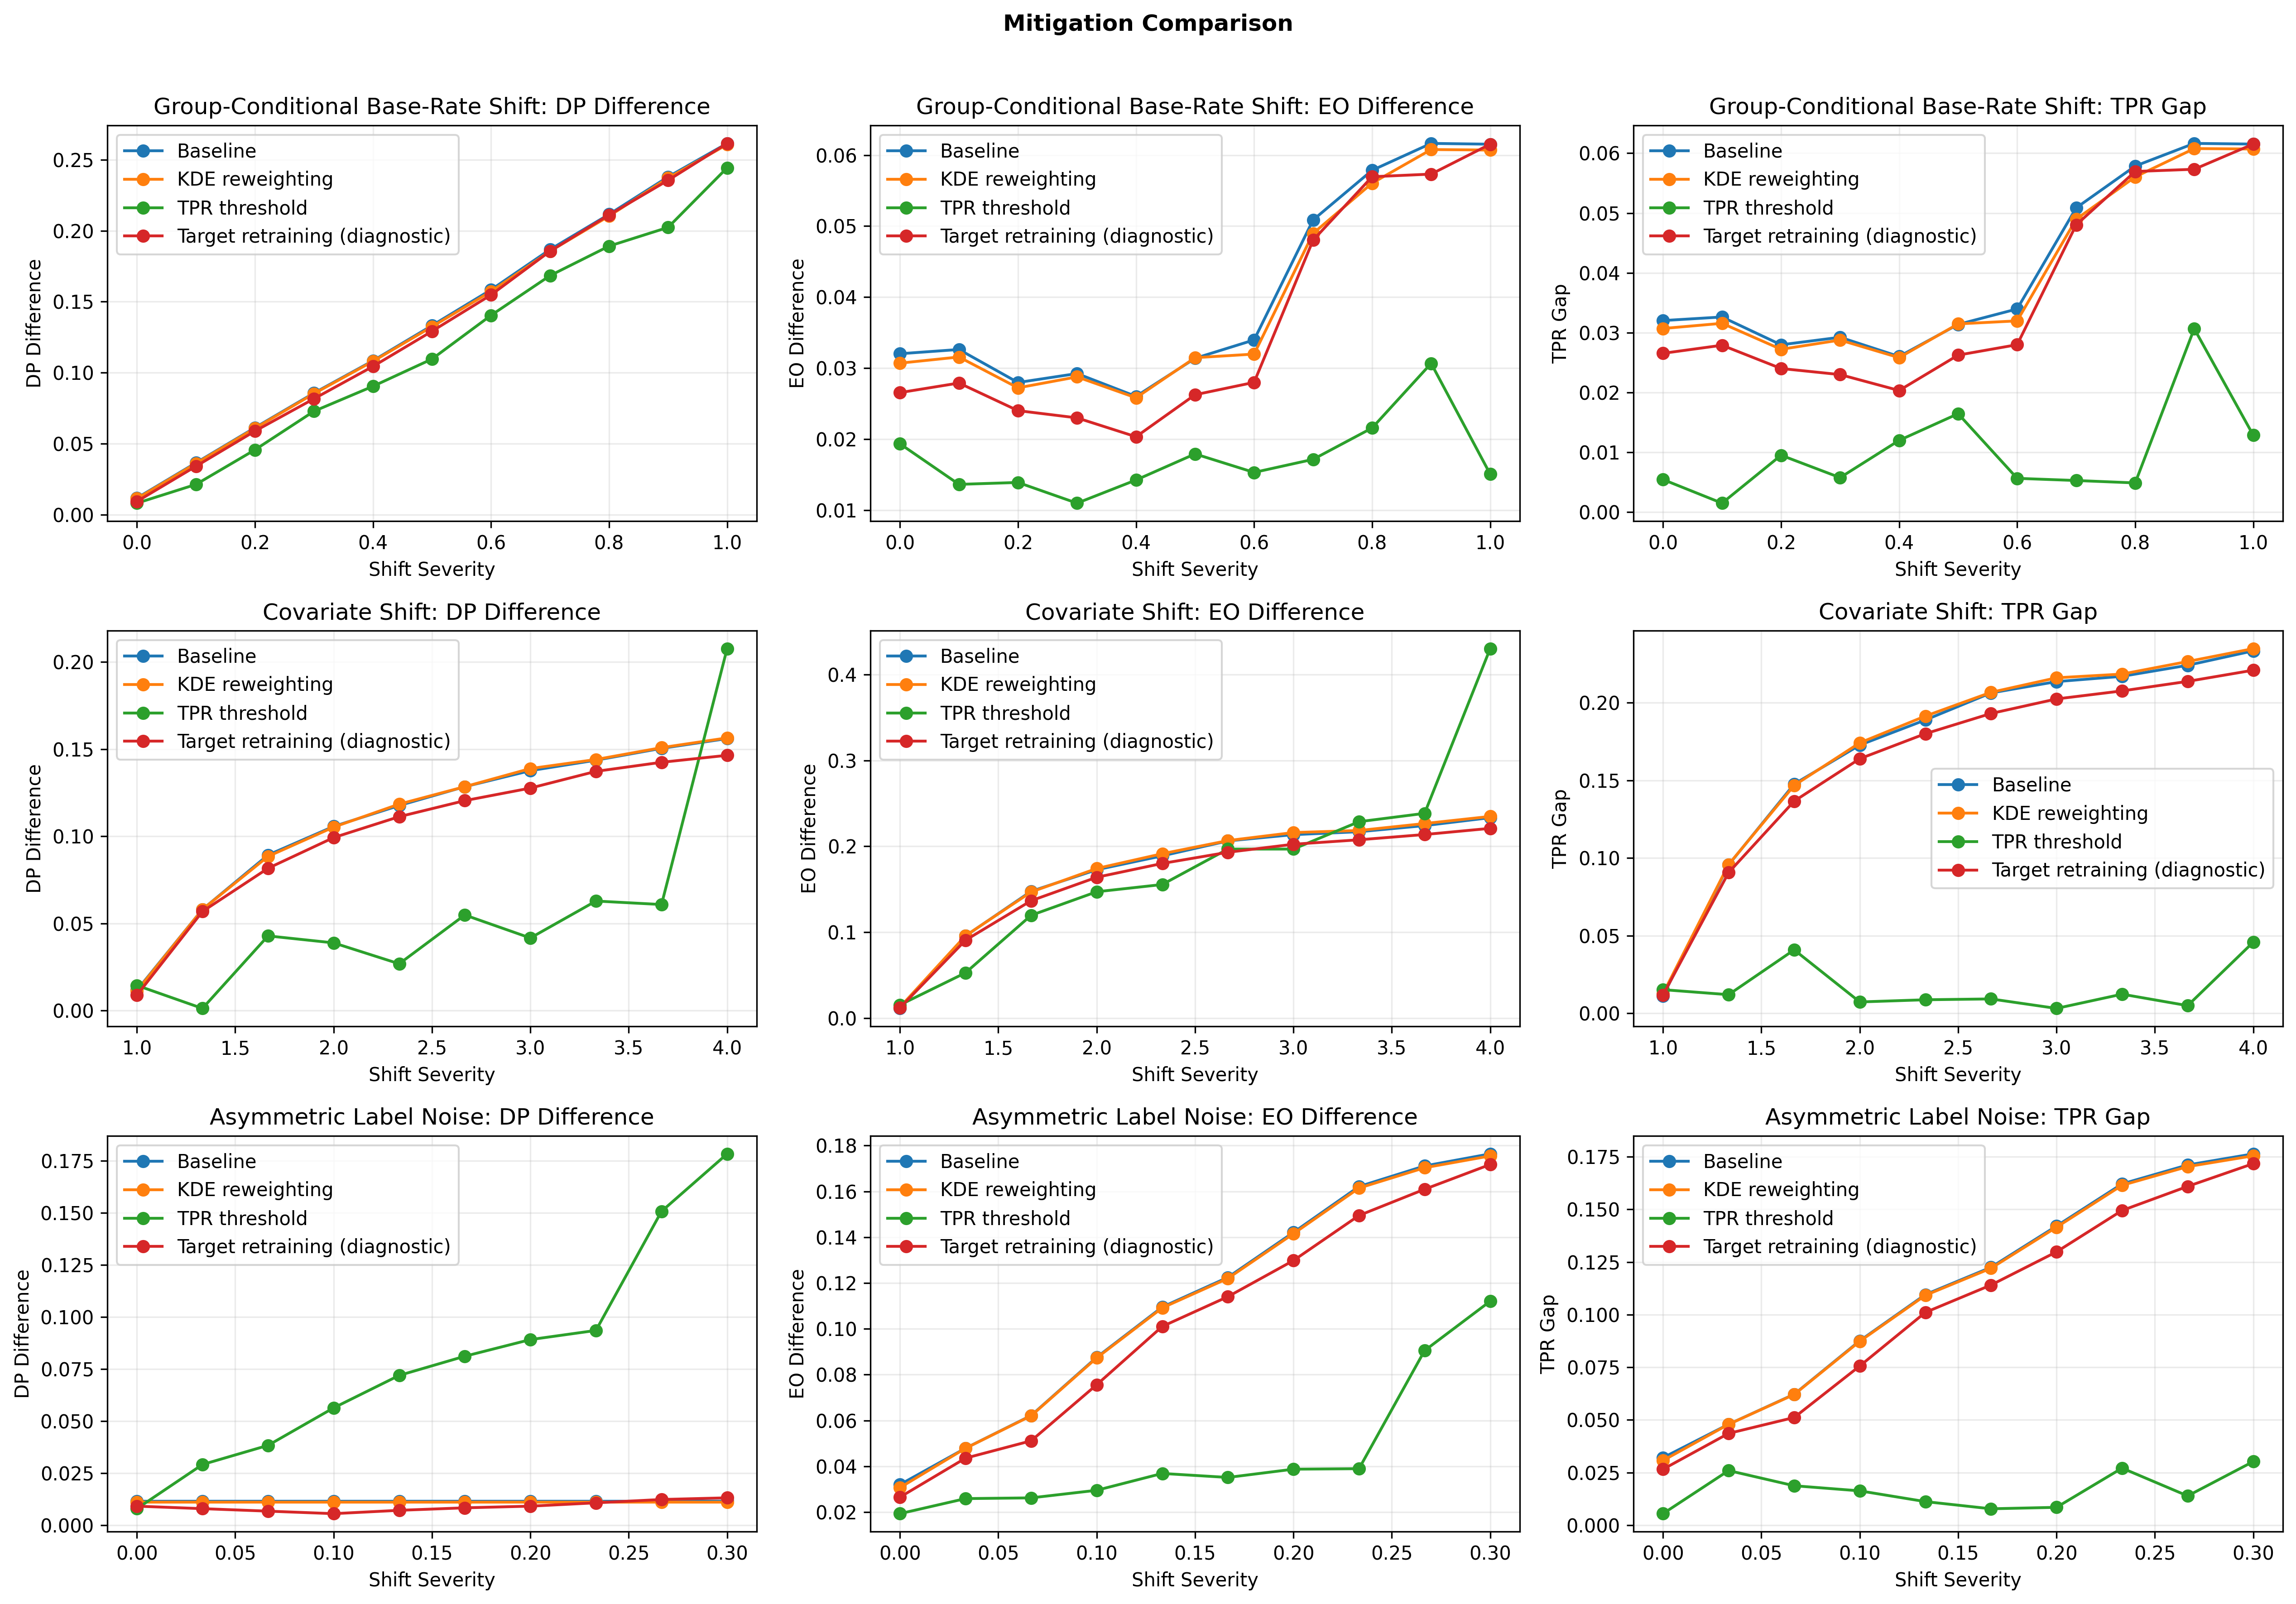
\includegraphics[width=0.87\textwidth]{mitigation_comparison.png}
\par\smallskip
{\scriptsize\itshape Figure S3: Three-seed mitigation comparison across shifts.}
\end{frame}

\begin{frame}
\frametitle{Results: KDE and Threshold Adjustment}
\centering
\includegraphics[width=0.88\textwidth]{mitigation_delta.png}
\par\smallskip
{\scriptsize\itshape Changes from the frozen model under KDE reweighting and threshold adjustment.}
\end{frame}

\begin{frame}
\frametitle{Results: Target Retraining}
\centering
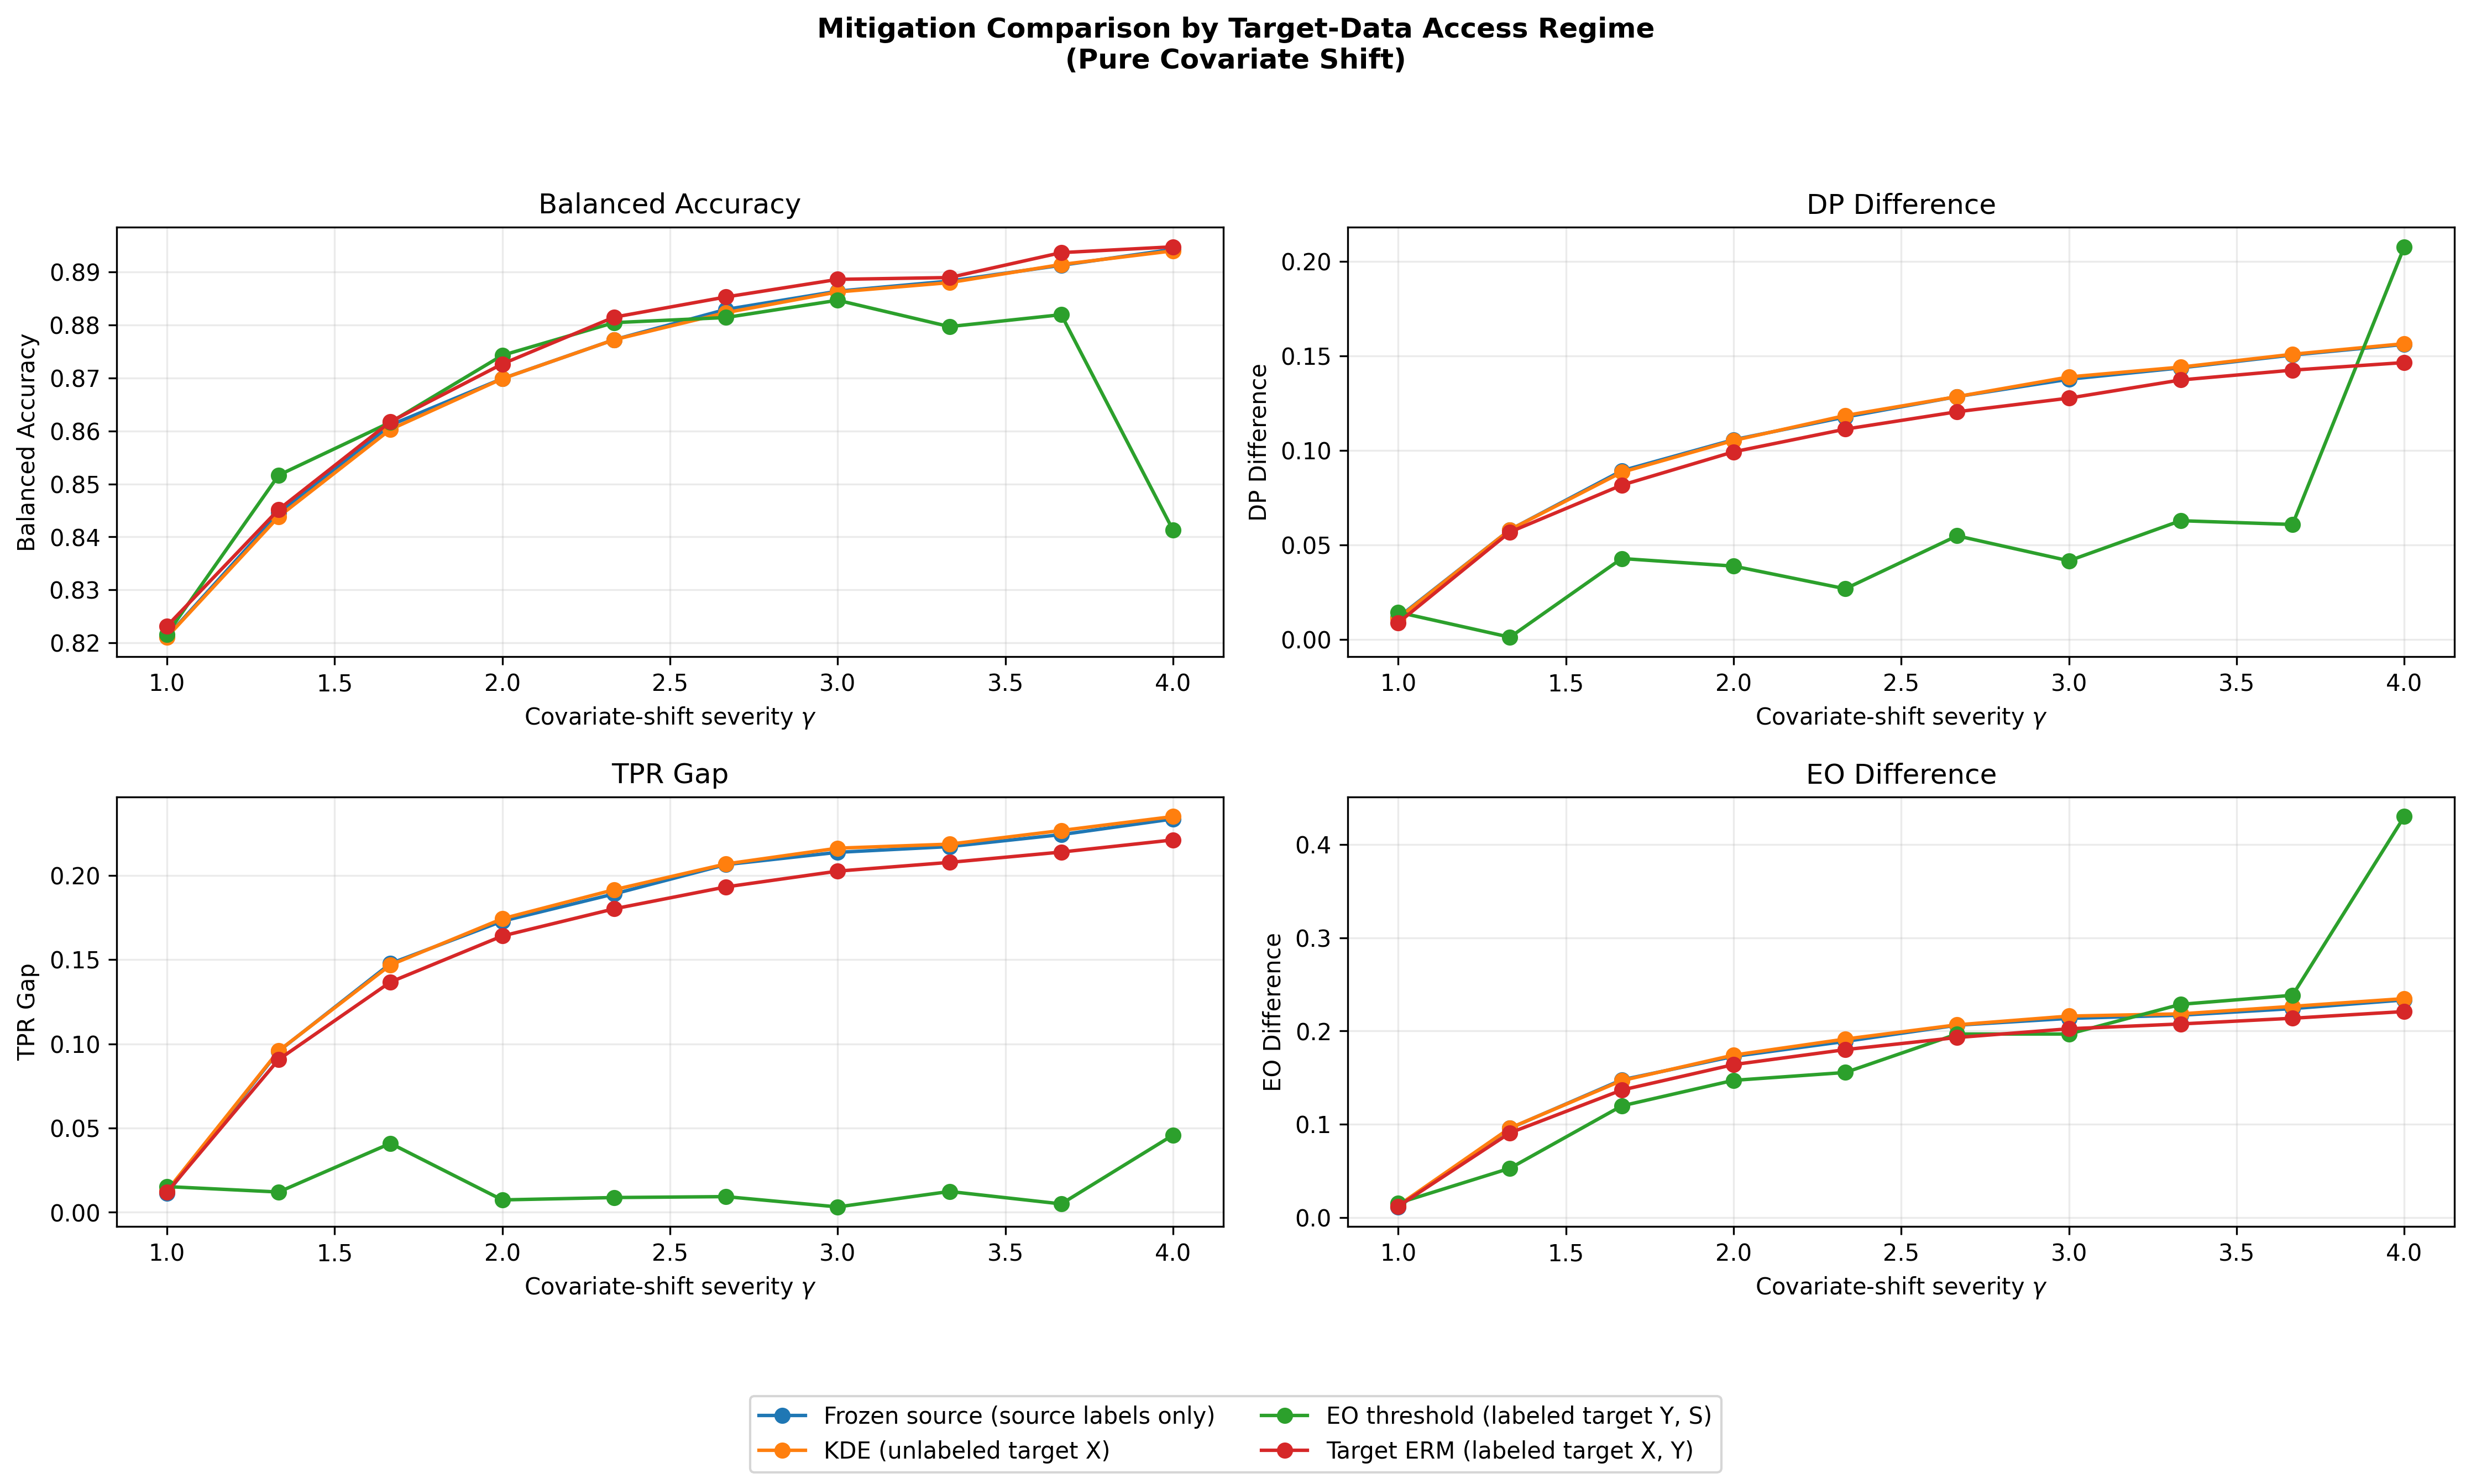
\includegraphics[width=0.87\textwidth]{mitigation_access_regimes_covariate.png}
\par\smallskip
{\scriptsize\itshape Figure S1: Mitigation under pure covariate shift, organized by target-data access.}
\end{frame}


\begin{frame}
\frametitle{Results: Key Empirical Findings (Part 2)---Mitigation}

\begin{itemize}
    \item \textbf{KDE Reweighting:}
    \begin{itemize}
        \item Under pure covariate shift, nearly coincides with the correctly specified frozen model (as expected).
        \item In other shift types, it serves as a negative control and does not improve fairness.
    \end{itemize}
    
    \item \textbf{Threshold Adjustment (Equal Opportunity):}
    \begin{itemize}
        \item Under covariate shift: reduces max TPR gap from $0.219$ to $0.044$, but max EO rises to $0.333$ (FPR gap grows).
        \item At $\gamma=4$, balanced accuracy drops from $0.893$ to $0.863$.
        \item Under label noise: raises DP from $0.014$ to $0.178$ (at $\beta=0.3$).
        \item \alert{Explicitly reducing TPR gap can increase DP or FPR-driven EO.}
    \end{itemize}
    
    \item \textbf{Target ERM:}
    \begin{itemize}
        \item Remains close to frozen model under pure covariate shift; not a universal fairness fix.
    \end{itemize}
\end{itemize}

\end{frame}


\begin{frame}
\frametitle{Discussion: Implications for Practice}

\begin{enumerate}
    \item \alert{A stable DP value can mask large changes in error-based fairness.}
    \begin{itemize}
        \item Asymmetric label noise is the clearest example.
        \item Dashboards monitoring only DP may miss or mischaracterize recorded-outcome disparities.
    \end{itemize}
    
    \item \alert{Error-based metrics can change sharply even when predictions are unchanged.}
    \begin{itemize}
        \item Under label noise, this can reflect measurement distortion rather than worse clean-outcome performance.
    \end{itemize}
    
    \item \alert{Conclusion depends on both metric and outcome definition.}
    \begin{itemize}
        \item Recorded vs. clean outcomes can produce entirely different conclusions.
        \item Data quality and documentation noise matter for fairness monitoring.
    \end{itemize}
\end{enumerate}

\begin{block}{Recommendation}
\small
  Track at least DP (referral volume), TPR gaps (missed necessary follow-up), 
  and calibration gaps (how equally clinicians can trust scores) side by side.
  Also audit outcome definitions for recording bias.
\end{block}

\end{frame}


\begin{frame}
\frametitle{Conclusion and Future Work}

\textbf{Key Takeaways:}

\begin{itemize}
    \item Stable DP can be misleading; error-based metrics and outcome definitions are essential.
    \item Mitigations have trade-offs and respect different data-access assumptions.
    \item \alert{Caution against over-interpreting any single fairness statistic as a stable "fairness guarantee"} after deployment shifts.
\end{itemize}

\vspace{0.5cm}

\textbf{Future Directions:}
\small
\begin{enumerate}
    \item Extend to richer feature spaces, multi-class, and causal outcome definitions.
    \item Wider uncertainty quantification and model families.
    \item Explore randomized equalized-odds post-processing.
\end{enumerate}

\end{frame}


\begin{frame}
\frametitle{References}

\small
\begin{enumerate}
    \item Asiaee, A., \& Aryan, K. (2026). Fairness under group-conditional prior probability shift: Invariance, drift, and target-aware post-processing. \textit{arXiv:2602.05144}.
    \item Chen, Y., Raab, R., Wang, J., \& Liu, Y. (2022). Fairness transferability subject to bounded distribution shift. \textit{arXiv:2206.00129}.
    \item Barrainkua, A., Gordaliza, P., Lozano, J. A., \& Quadrianto, N. (2022). A survey on preserving fairness guarantees in changing environments. \textit{arXiv:2211.07530}.
    \item Shao, M., Li, D., Zhao, C., Wu, X., Lin, Y., \& Tian, Q. (2024). Supervised algorithmic fairness in distribution shifts: A survey. \textit{arXiv:2402.01327}.
\end{enumerate}
\end{frame}

\end{document}
